\documentclass{article}
\usepackage[utf8]{inputenc}

\title{ECS 145 Term Project}
\author{Gavin Grey, Jeremy Kwan, Shayan Mandegarian, Michael Nguyen}
\date{}

\usepackage{natbib}
\usepackage{graphicx}

\begin{document}

\maketitle

\section{Introduction}
For our term project, we had to write a function of call form exploreShape(x, estMethod, tuning, twoAtATime) where x is a numeric vector, estMethod is whether we want to graph a histogram or a density graph, tuning is the number of breaks we have in the graph, and twoAtATime is whether we want to superimpose the previous graph onto a new graph.


\section{Graphing}

\begin{figure}[h!]
\centering
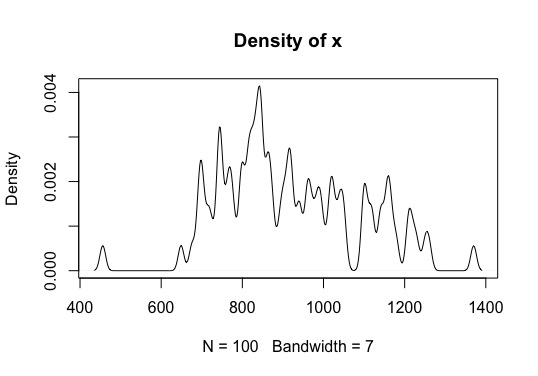
\includegraphics[scale=0.5]{Nile, 7 Tuning param.jpeg}
\caption{Sample output explore(Nile, 'density', 7, T)}
\label{fig:Nile density graph}
\end{figure}

Whenever we change the tuning parameter of the graph, if twoAtATime is initialized as true, then the previous graph is kept and superimposed onto the other graph. The previous graph is colored red to help differentiate between the graphs.

\begin{figure}[h!]
\centering
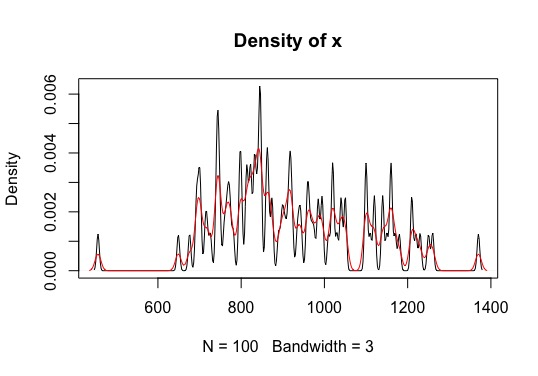
\includegraphics[scale=0.5]{Nile, 7 superimposed on 3.jpeg}
\caption{Sample output explore(Nile, 'density', 7, T) and then changing tuning parameter to 3. }
\label{fig:Nile density graph}
\end{figure}


%\section{Conclusion}
%``I always thought something was fundamentally wrong with the universe'' %\citep{adams1995hitchhiker}

%\bibliographystyle{plain}
%\bibliography{references}

\end{document}
